
\documentclass{IOS-Book-Article}

\usepackage{mathptmx}
\usepackage{subcaption}
\usepackage{times}
\usepackage{CJKutf8}
\usepackage{mathrsfs}
\usepackage{textcomp}
\usepackage{verbatim}
\usepackage{amsmath}
\usepackage{amsfonts}
\usepackage{xspace}
\usepackage{xcolor}
\usepackage{url}
\usepackage{balance}
\usepackage{booktabs}
\usepackage{multirow}
\usepackage{rotating}
\usepackage{fancyvrb}
\usepackage{lastpage}
\usepackage{alltt}
\usepackage{etoolbox}
\usepackage{cleveref} % After hyperref, listings
\usepackage{fancyhdr}
\usepackage{listings}
\usepackage{caption}

%\usepackage{times}
%\normalfont
%\usepackage[T1]{fontenc}
%\usepackage[mtplusscr,mtbold]{mathtime}
%
\def\hb{\hbox to 10.7 cm{}}

\begin{document}

\pagestyle{headings}
\def\thepage{}

\begin{frontmatter}              % The preamble begins here.


%\pretitle{Pretitle}
\title{Optimizing Performance and Scalability of Google Tensorflow on Manycore
CPU}
%\markboth{}{September 2016\hb}
%\subtitle{Subtitle}
%\author[A]{\fnms{Book Production} \snm{Manager}%
%\thanks{Corresponding Author: Book Production Manager, IOS Press, Nieuwe Hemweg
% 6B, 1013 BG Amsterdam, The Netherlands; E-mail:
%bookproduction@iospress.nl.}},
%\author[B]{\fnms{Second} \snm{Author}}
%and
%\author[B]{\fnms{Third} \snm{Author}}

%\runningauthor{B.P. Manager et al.}
%\address[A]{Book Department, IOS Press, The Netherlands}
%\address[B]{Short Affiliation of Second Author and Third Author}

\begin{abstract}
We propose an optimization method for Google Tensorflow on a single
shared-memory manycore architecture using a new CPU optimizing method and
an efficient memory placement method to improve performance scalability.
The performance problems of Tensorflow frameworks have only considered on large
distributed clusters with GPUs resulting from the cluster-based
algorithms that only focused on avoiding high network costs and improving GPU
performance. 
However, some of large scale machine learning data sets can be processed with a
single commodity manycore machine instead of using distributed clusters with
GPUs since shared-memory manycore machine can reduce network and PCI-E
bus transfers.
The proposed methods can improve performance and scalability on the unoptimized
Tensorflow with a single manycore machine by using efficient vectorization,
maximizing the CPU utilization and efficient memory placement.
Our method will provide the basis towards practical design of deep learning
framework for a single manycore server to collaborate CPUs and GPUs. 
Our evaluation study based on benchmark programs revealed that our optimizing
method will show better performance improvement through on a 64 core Intel
Xeon-phi KNL, self-bootable single manycore CPUs, compared to unoptimized
Tensorflow.
\end{abstract}

\begin{keyword}
Mayncore\sep Tensorflow\sep Intel Xeon-phi KNL\sep 
\end{keyword}
\end{frontmatter}
%\markboth{September 2017\hb}{September 2016\hb}
%\thispagestyle{empty}
%\pagestyle{empty}


\section{Introduction}
In recent years, deep learning has produced several domains ranging from speech
recognition, visual object recognition, to text processing.
However, deep learning data sets have substantially grown during the last
decade. 
To solve large data sets, the current design trend is to use large-scale
clusters of machines, which is distribute training and inference in deep
networks using the state of the art deep learning frameworks.

Google Tensorflow~\cite{Abadi2016TSL} is one of widely used deep learning
analytics framework to solve large data sets problem, and it becomes more and
more a versatile framework for distributed clusters, local workstations, mobile
devices, and custom-designed accelerators.
However, Tensorflow does not scale on the single manycore machine resulting
from our preliminary experiments (see Section 2) because Tensorflow was the
successor to DistBelief~\cite{Dean2012LSD}, a heavyweight system, and it only
added support for GPU acceleration~\cite{Abadi2016TSL}.

A. Matveev \textit{et al.} proposed a deep learning algorithm and CPU
optimizing methods that eliminate the bottleneck of transferring data to the
cloud thereby reducing the transferring overheads~\cite{Matveev2017MPC}.
Therefore, we also believed that some of workloads on a single manycore machine
can perform faster than a distributed clusters of CPUs and GPUs, so CPU scaling
problem server must be solved on Tensorflow.
Our optimizing method will provide the basis towards practical design to
collaborate CPUs and GPUs.

\begin{figure*}[tb]
    \centering
    \begin{subfigure}[b]{0.5\textwidth}
        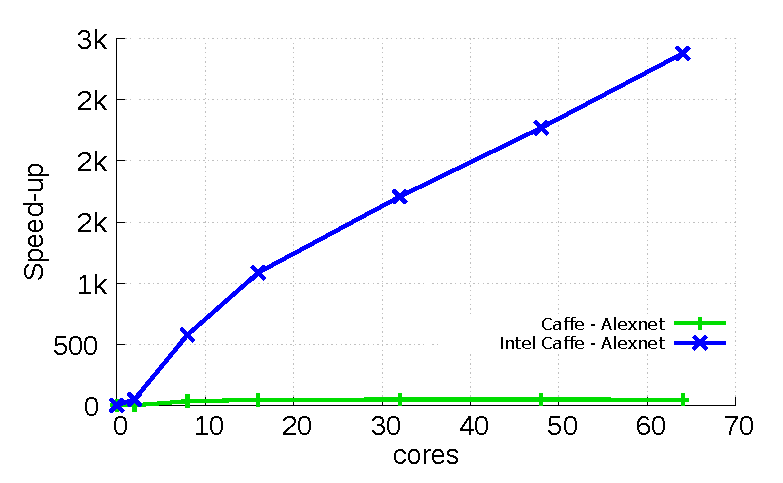
\includegraphics[width=2.3in]{graph/caffe.eps}
        \caption{Scale-up server scalability of Caffe}
    \end{subfigure}%
    \begin{subfigure}[b]{0.5\textwidth}
        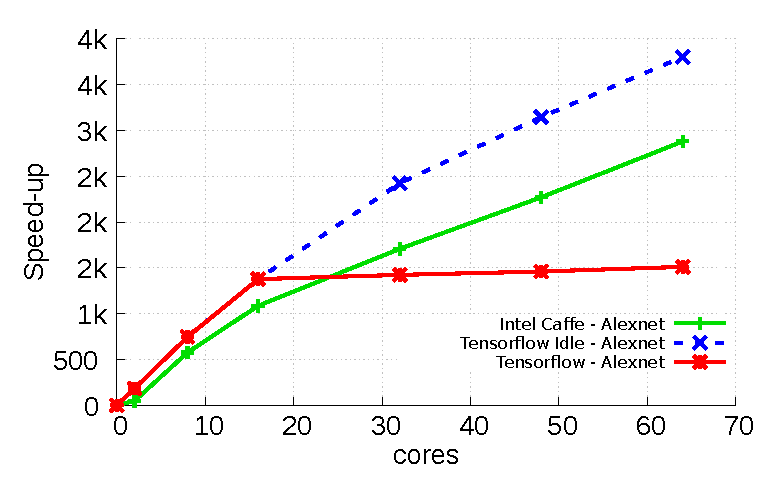
\includegraphics[width=2.3in]{graph/tensorflow.eps}
        \caption{Scale-up server scalability of Tensorflow}
    \end{subfigure}%
    \label{fig:scalability}
\end{figure*}


\section{Preminerly Expermiments}
As noted earlier, Tensorflow does not scale on the single manycore machine. 
In order to achieve the high performance on Tensorflow, we need to understand
the problem of Tensorflow on a single manycore machine. 
Figure~\ref{fig:scalability} (a) explains the improving point of
original Caffe on Intel Xeon-phi KNL; original Caffe didn’t scale well. 
On the other hand, Intel optimized Caffe on Intel Xeon-phi KNL processor 
improved the performance scalability significantly.
However, until recently, Figure ~\ref{fig:scalability} (b) shows that Tensorflow
has not been optimized on Intel Xeon-phi KNL processor due to the it does not
support CPU optimization technique such as OpenMP and Intel MKL library.
This results show us to problem of performance and scalability on a single
manycore machine.

\section{Proposed Methods}
In order to achieve the high performance and scalability on a single manycore
machine, we may use a method to optimize vectorization, multithreading, and
better cache traffic.
In conclusion, optimizing CPU performance and scalability on Tensorflow can
replace the use of a larget distributed system with a single manycore machine
through benefits of the low shared-memory communication overheads, and
parallelize.
This is the main focus of our research and implementation.

\bibliographystyle{abbrv}
\bibliography{ref}
 
%\begin{thebibliography}{99}
%\bibitem{r1}
%\textit{Scientific Style and Format: The CBE manual for authors,
%editors and publishers}. Style Manual Committee, Council of Biology Editors.
%Sixth ed. Cambridge University Press, 1994.

%\bibitem{r2}
%L.U. Ante, Cem surgere: Surgite postquam sederitis, qui manducatis panem
% doloris, \textit{Omnes} \textbf{13} (1916), 114--119.

%\bibitem{r3}
%T.X. Confortavit, \textit{Seras}, Portarum, New York, 1995.

%\bibitem{r4}
%P.A. Deus, Ater hoc et filius et mater praestet nobis,
%\textit{Paterhoc} \textbf{66} (1993), 856--890.

%\end{thebibliography}

\end{document}
